\section{Introduction}
\label{sec:intro}

Writing a Geant4\cite{geant4} simulation code without hardcoded numbers is
as easy as replacing calls like \verb|G4Box(‘box’, 20, 30, 40)| with
code such as~\verb|G4Box(name, a, b, c)|
where the parameters are read from a database, for example mysql.
This however is not particularly useful: users still need to write C++ and Geant4 code to setup
the volumes definitions organization, sensitivity, how to digitized the Geant4 steps
and collect them into hits saved in some output format.

\begin{figure}[h]

    \centering
    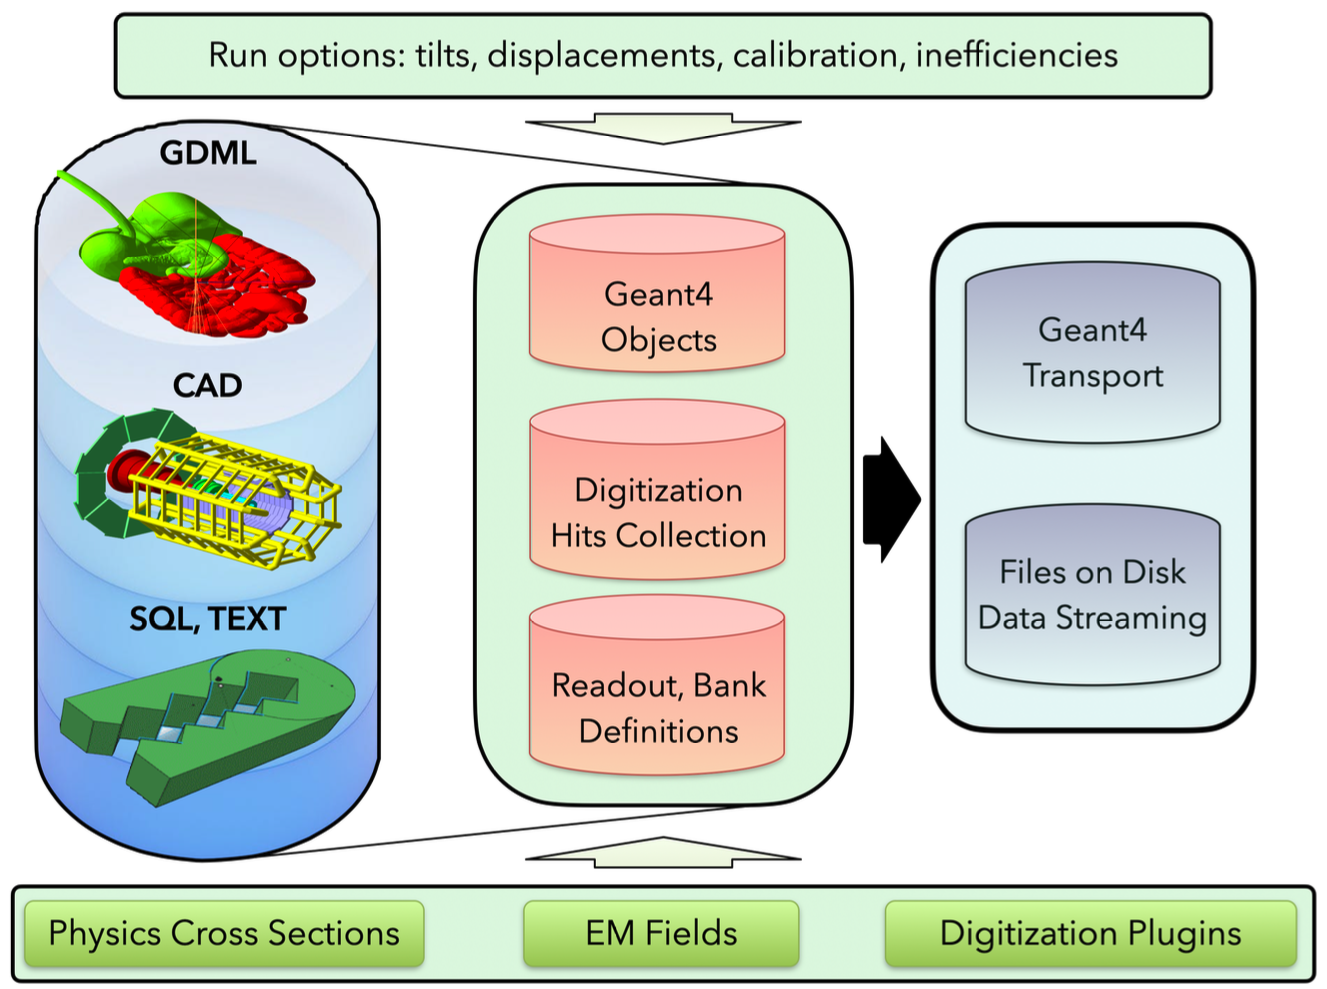
\includegraphics[width=.90\textwidth]{img/db}
    \caption{A Geant4 application driven in its entirety by a database: geometry, materials,
        digitization, readout electronics, output format.}
    \label{fig:db}
\end{figure}

A program such as the one sketched Fig.\ref{fig:db}, capable of build Geant4 objects from a database
and run the simulation present several advantages, among which:

\begin{itemize}
    \item no pre-requisite knowledge of c++ or Geant4 required to write the simulation
    \item the experiment setup is naturally shared among different users, without the need to re-compile  the code
    \item the same application can be used to simulate different experiments, by simply
    selecting the desired setup from the database
\end{itemize}
We present the database driven GEMC\cite{clas12_gemc} application.  It provides:

\begin{itemize}
    \item a python API to build detectors and populate the databases
    \item hardware emulation of the readout electronics
    \item user defined digitization of the Geant4 steps
    \item data streaming to disk or network
\end{itemize}


\section{Features}
\label{sec:features}

\subsection{Databases}
\label{subsec:databases}

\subsection{Python API}
\label{subsec:api}

\subsection{Electronic Time Window}
\label{subsec:time_window}

\subsection{Energy Sharing}
\label{subsec:energy_sharing}

\subsection{Digitization}
\label{subsec:digitization}

\subsection{Data Streamer}
\label{subsec:data_streamer}


\section{Examples}
\label{sec:examples}

\subsection{Cad Import}
\label{subsec:cad_import}

\subsection{Flux scintillator paddle}
\label{subsec:flux_scintillator_paddle}

\subsection{GEMC at Jefferson Lab}
\label{subsec:clas12}


\section{Summary}
\label{sec:summary}

